\documentclass[chapterprefix=false, 12pt, a4paper, oneside, parskip=half, listof=totoc, bibliography=totoc, numbers=noendperiod]{scrbook}

\usepackage[utf8]{inputenc}
\usepackage[T1]{fontenc}
\usepackage[bottom=48mm,left=25mm,right=25mm]{geometry}
\usepackage[onehalfspacing]{setspace}
\usepackage[stretch=10]{microtype}
\usepackage{xcolor}
\usepackage{scrhack}
\usepackage{titling}
\usepackage[outputdir=out]{minted}
\usepackage{graphicx}
\usepackage{hyperref}
\usepackage[ngerman]{babel}

\renewcommand*{\chapterheadstartvskip}{\vspace*{.25\baselineskip}}
\def\changemargin#1#2{\list{}{\rightmargin#2\leftmargin#1}\item[]}
\let\endchangemargin=\endlist

\definecolor{htwgruen}{RGB}{118, 185, 0}
\definecolor{htwblau}{RGB}{0, 130, 209}
\definecolor{htworange}{RGB}{255, 95, 0}
\definecolor{htwgrau}{RGB}{175, 175, 175}


\title{Bericht über Werkstudententätig bei der DERICON GmbH}
\author{Christoph Stach}
\date{01.11.2016 bis 30.09.2018}


\begin{document}
    \begin{titlepage}
		% Logo
        
\includegraphics[width=0.50\textwidth]{img/Q01_HTW_Berlin_Logo_quer_pos_FARBIG_CMYK.eps}

        % Abstand nach logo
        \vspace{4.0cm}

        % Textkörper
        \begin{changemargin}{0.5cm}{0.0cm}
        % Dokumenttyp
        \color{htwgrau}
        \normalsize
        \textsf{\noindent\MakeUppercase{Dokumenttyp}} \vspace{-20pt}\\
        % Horizontale Linie
        \noindent\rule{\textwidth}{0.5pt}\vspace{-4pt}
        % Title
        \color{black}
        \huge
        \textsf{Bericht über Werkstudententätig}
        \vspace{12pt}

        % Author
        \color{htwgrau}
        \normalsize
        \textsf{\MakeUppercase{Author}}\\
        \color{black}
        \large
        \textsf{\theauthor}

        % Zeitraum
        \color{htwgrau}
        \normalsize
        \textsf{\MakeUppercase{Zeitraum}}\\
        \color{black}
        \large
        \textsf{\thedate}

        % Am Ende der Seite
        \vfill

        % Firma
        \color{htwgrau}
        \normalsize
        \textsf{\MakeUppercase{Firma}}\\
        \color{black}
        \large
        \textsf{DERICON GmbH}

        % Dozent
        \color{htwgrau}
        \normalsize
        \textsf{\MakeUppercase{Dozent}}\\
        \color{black}
        \large
        \textsf{Prof. Dr. Schüler}
        \vspace{-60pt}
        \end{changemargin}
    \end{titlepage}

    \tableofcontents

    \chapter{Allgemeines}

    Dieser Bericht behandelt die Werkstudententätigkeit von Christoph Stach bei der DERICON GmbH im Zeitraum vom 01.10.2016 bis 31.09.2018.

    \section{Beschreibung des Unternehmens}

    Die DERICON GmbH ist ein bankenunabhängiges Finanzdienstleistungsinstitut mit Standorten in Frankfurt am Main und Berlin.
    Das Unternehmen unterstützt seit 2008 Banken und Vermögensverwalter bei der Gestaltung effizienter und rechtskonformer Beratungs- und Vertriebsprozesse.
    Mit DERIFIN betreibt DERICON dafür die führende Webanwendung zur Selektion, Steuerung und Risikomanagement von strukturierten Produkten.
    Zudem liefert DERICON professionelle Daten und Kennzahlen für die Analyse und den Einsatz strukturierter Produkte.
    Europaweit vertrauen bereits mehr als 60 Privatbanken, Sparkassen und Genossenschaftsinstitute auf die Expertise von DERICON.
    \\ \\
    Im Jahr 2015 wurde über DERIFIN ein Anlagevolumen von rund 1,2 Mrd. Euro vermittelt.

    \section{Beschreibung der Produkte}

    Das Hauptprodukt von DERICON ist die Webanwendung DERIFIN. Außerdem wurde während ich bei der DERICON GmbH eingestellt war,
    eine neue Version von DERIFIN entwickelt, das sogennante DERIFIN WMS. Welches mehr Features bietet und mit neueren Technologien entwickelt wurde.
    Neben der Hauptsoftware DERIFIN entwickelt DERICON viele internete Produkte zur besseren Verwaltung von DERIFIN und seiner Kunden.

    \section{Beschreibung des Teams}

    Das Team von DERICON ist auf zwei Standorte verteilt. Der erste Standort ist in Frankfurt am Main und der zweite Standort in Berlin Charlottenburg.
    Mein Arbeitsplatz ist im Berliner Büro. Zum heutigen Zeitpunkt arbeiten zwei Frontend-Entwickler, sowie einer der Geschäftsführer in diesem Büro.
    Im Frankfurter Büro arbeiten überwiegend Backend-Entwickler sowie ein weiterer Geschäftsführer und die Buchhaltung.
    \\ \\
    Die komplette Entwicklungsabteilung hält jeden Morgen ein Meeting per Videotelefonie, in dem jedes Mitglied kurz berichtet
    was er am Vortag gemacht hat und was er an diesem Tag vorhat.
    Die Entwicklung ist in Sprints von zwei Wochen gegegliedert. Deswegen gibt es ein weiteres Sprintplanungsmeeting am Anfang eines jeden Sprints.
    Dieser Prozess ist an \footnote{Eine Methode für agiles Projektmanagement.}SCRUM angelehnt.

    \section{Organisation}

    \subsection{Issue-Management}

    Die Aufgabenverteilung ist über die Software \footnote{Eine Webanwedung für das Projektmanagement und die Fehlerverwaltung von Software. \\ Link: \url{https://www.atlassian.com/software/jira}}JIRA geregelt.
    Alle neuen Features sowie anfallende Bugs werden hier gespeichert.
    Bei der Sprintplanung wird besprochen welche \footnote{In Jira werden Fehler, Features und andere Artefakte generell als Issues bezeichnet.}Issues
    im kommenden Sprint umgesetzt werden sollen. Die Issues werden über den Sprint hinweck vom Teamleader an die einzelnen Entwickler verteilt. Auch ist es möglich sich selbst Issues zuzuweisen.
;-
    \pagebreak

    \subsection{Versionskontrolle}

    Alle Software Projekte werden auf in \footnote{Eine Versionskontrollsystem entwickelt von Linus Torvalds. Link: \url{https://git-scm.com}}GIT-Repositories auf \url{https://bitbucket.org} gespeichert. Wird ein Issue aus JIRA von einem
    Entwickler fertiggestellt, wird auf Bitbucket ein Pullrequest auf den Development-Branch erstellt. Dieser muss erst von anderen Entwicklern überprüft werden, bevor er in entgültig in den Development-Branch der Software
    gemerged wird.

    \subsection{Buildmanagement}

    Alle Applikationen werde über \footnote{Ein Server zur Automatisierung von Aufgaben, wird oft für den Build-Prozess von Software eingesetzt. Link: \url{https://jenkins.io}}JENKINS gebaut,
    treten keine Fehler auf beim Buildprozess auf, werden diese danach von JENKINS auf die Server bei \footnote{Hostingservice für Server und andere Services der Firma Amazon. Link: \url{https://aws.amazon.com}}Amazon AWS kopiert.

    \chapter{Aufgaben}

    Während meiner Zeit bei der DERICON GmbH habe ich überwiegend an drei verschiedenen Softwareprodukten gearbeitet.
    Meine Arbeit bezog sich meistens auf die Implementierung neuer Features und dem Beheben von Fehlern.

    \section{CitrusNG}

    \subsection{Ausgangsposition}

    CitrusNG war das erste Projekt an dem ich mitgewirkt habe. Es ist ein internes Produkt für die Konfiguration der unterschiedlichen DERIFIN umgebungen, die
    vom Kunden benutzt werden. Jeder Kunde hat unterschiedliche Wünsche deswegen ist die DERIFIN Software sehr stark konfigurierbar, um die Konfigurationen einfacher
    zu verwalten gibt es CitrusNG.

    \pagebreak

    CitrusNG ist eine Webanwendung. Das Frontend ist mit \footnote{Link: \url{https://angularjs.org}}AngularJS (Version 1) implementiert. Das Backend mit SpringBoot Micro-Services.
    Zwischen Backend und Frontend wird eine weitere PHP-Ebene, mit \footnote{Symfony ist ein weitverbreitetes PHP Framework mit wiederverwendtbaren Bibliotheken und Komponenten der Firma SensioLabs. Link: \url{https://symfony.com}}Symfony 2 implementiert, in Form einer Middleware eingesetzt.
    Die Middleware sowie das Frontend wird von den Frontent-Entwicklern gepflegt.
     Das Ziel der Middleware ist es den Frontend-Entwicklern die Möglichkeit zu geben, die Ergebnisse der
    Backend-Endpunkte zu manipulieren und sie angepasst an das Frontend weiterzuleiten. Hier werden beispielsweise unötige JSON-Felder entfernt oder
    aggregiert, Mock-Daten generiert oder Sortierfunktionen implementiert.

    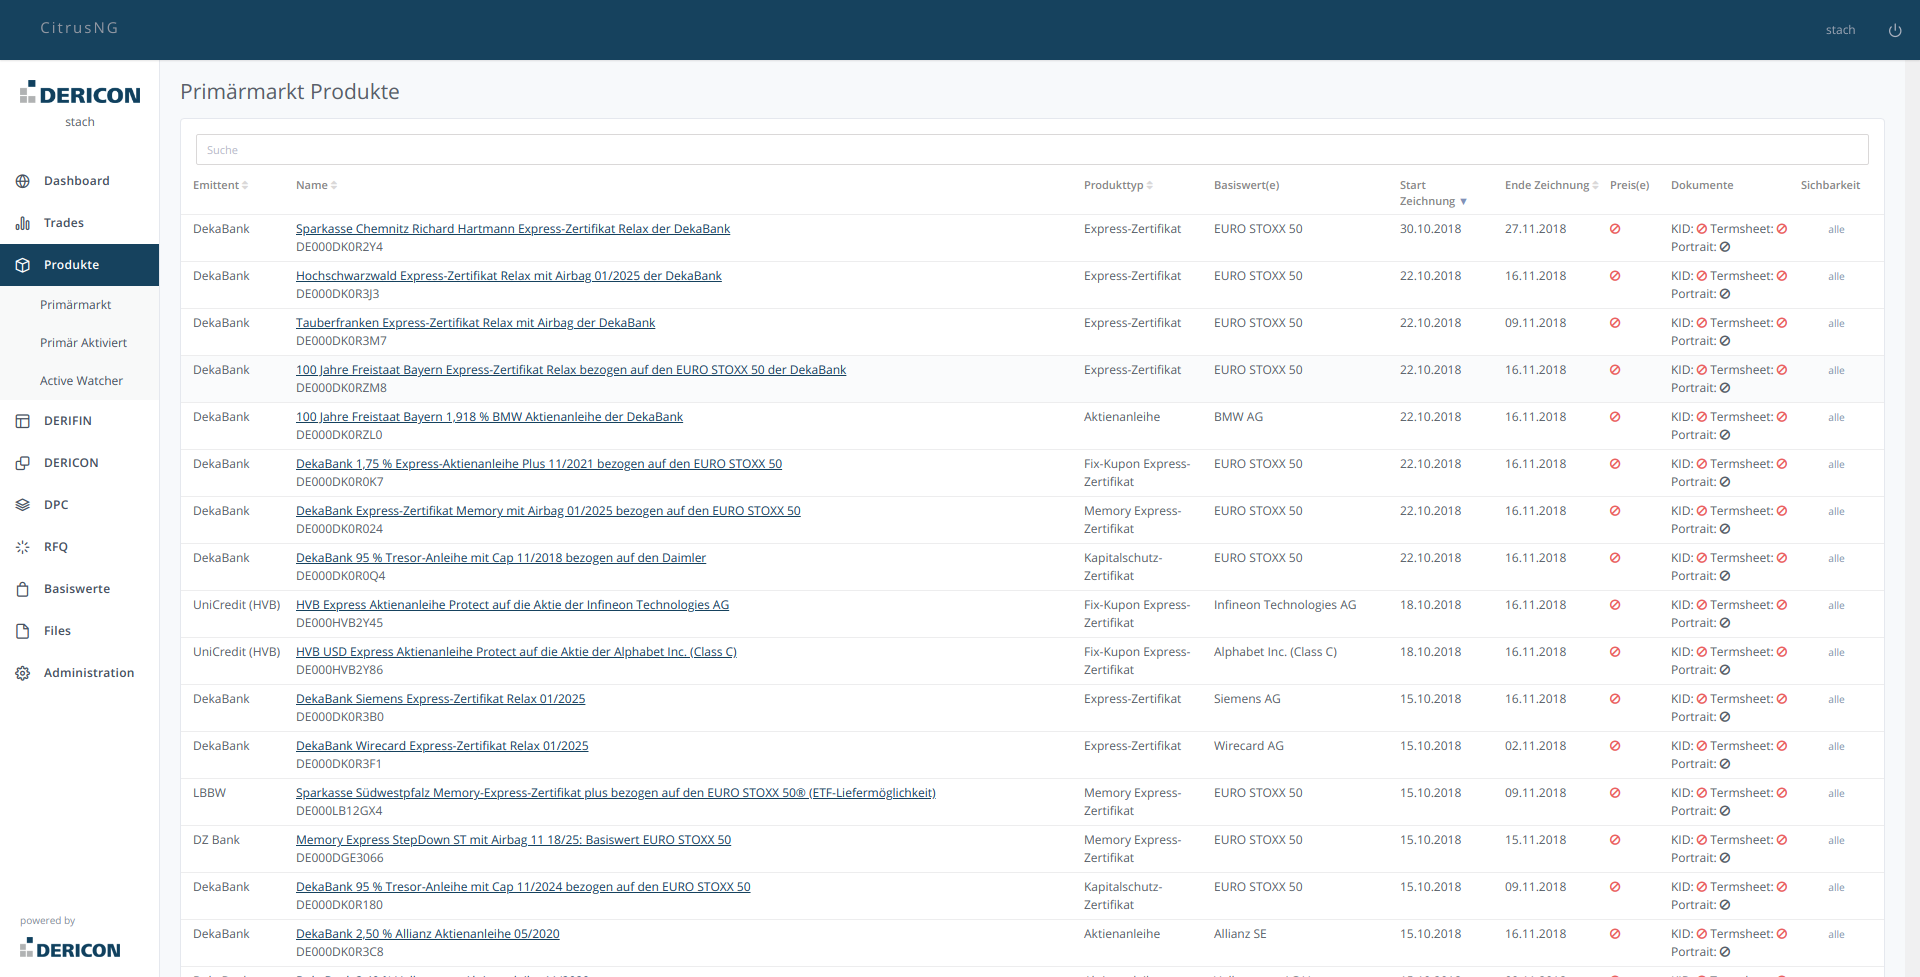
\includegraphics[width=1.00\textwidth]{img/citrusng.png}
    \captionof{figure}{Screenshot der Software CitrusNG}

    \subsection{Entwicklung}

    \subsection{Ergebnisse}

    \section{BrokerUI}

    \subsection{Ausgangsposition}

    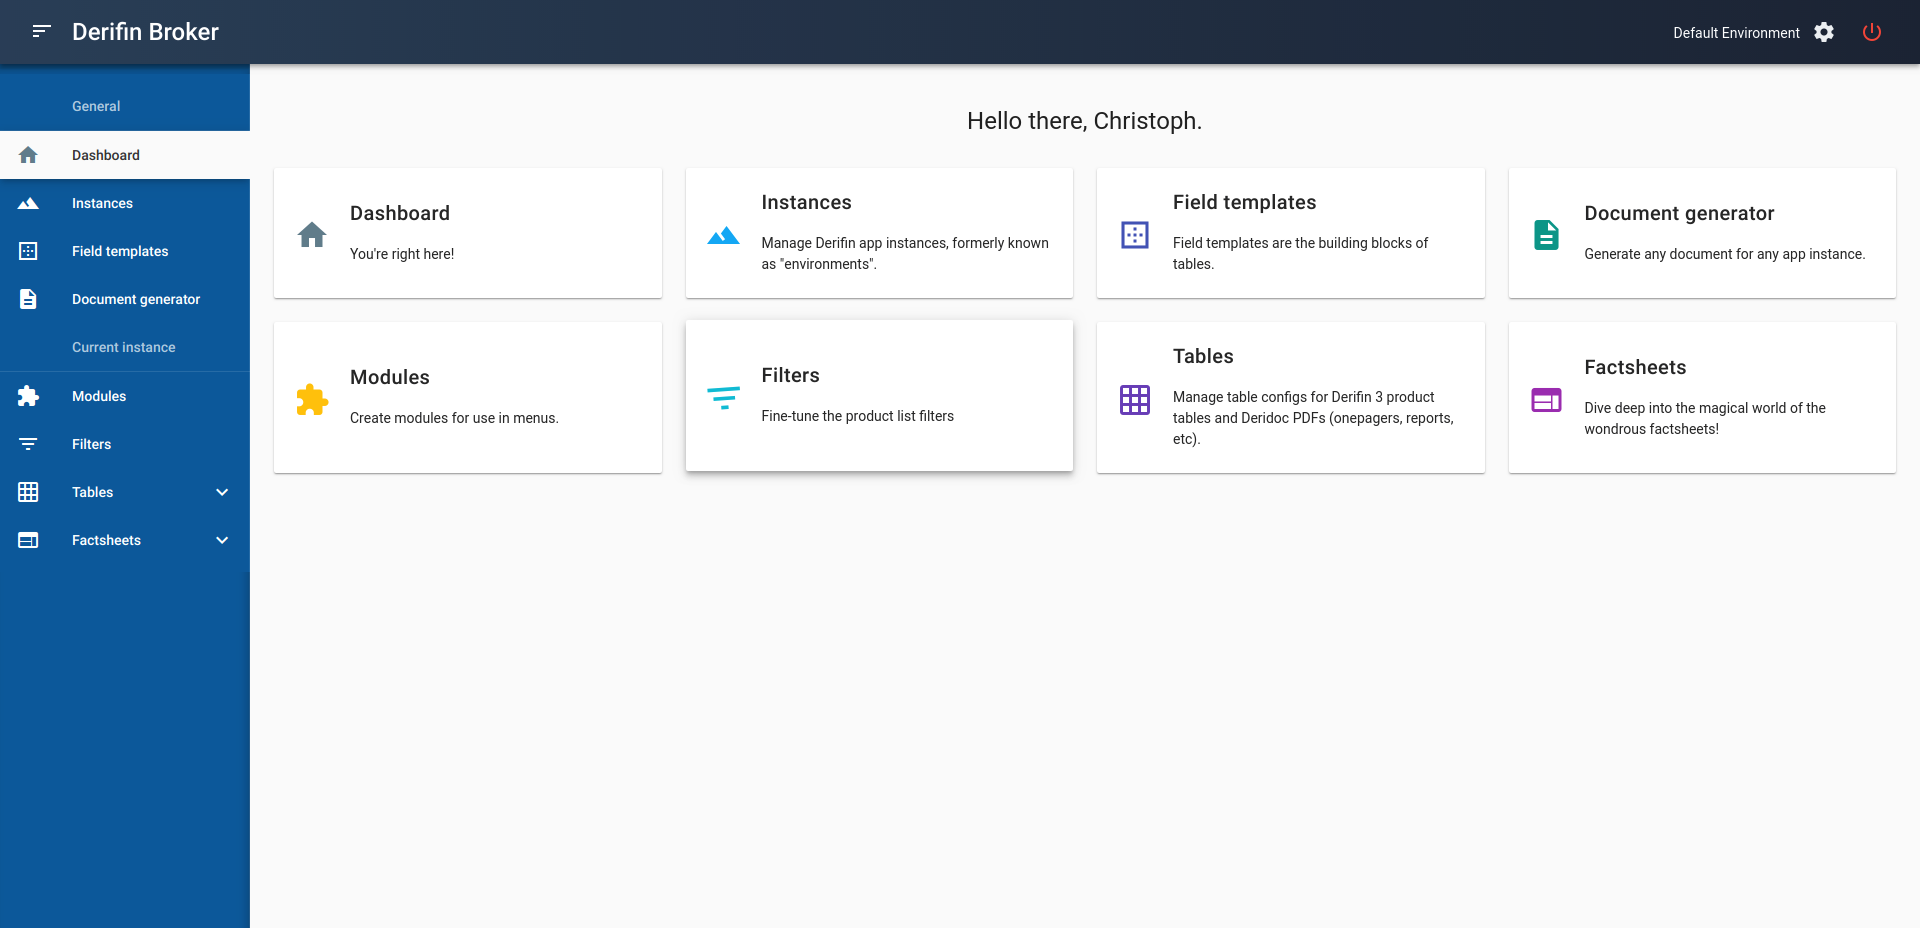
\includegraphics[width=1.00\textwidth]{img/broker-ui-neu.png}
    \captionof{figure}{Screenshot der Software BrokerUI}


    \subsection{Entwicklung}

    \subsection{Ergebnisse}

    \section{DERIFIN WMS}

    \subsection{Ausgangsposition}

    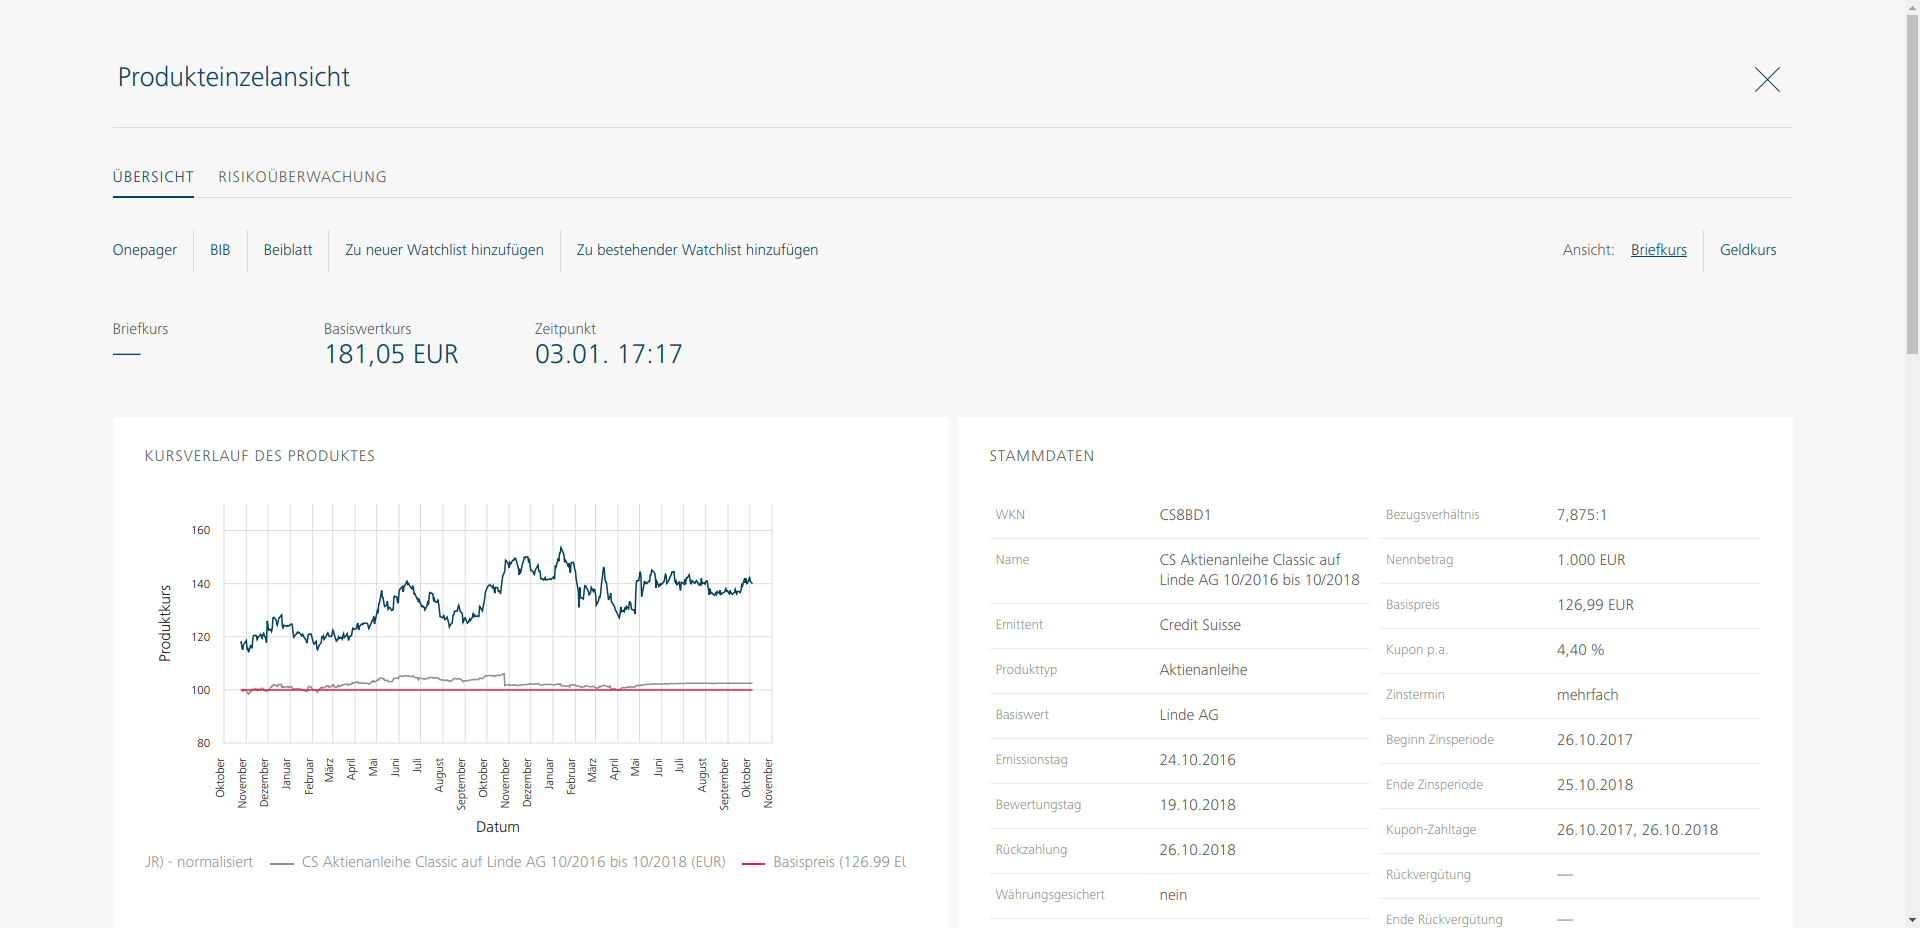
\includegraphics[width=1.00\textwidth]{img/derifin.png}
    \captionof{figure}{Screenshot der Software DERIFIN WMS}

    \subsection{Entwicklung}

    \subsection{Ergebnisse}

    \chapter{Schlussfolgerungen}

    \section{Zusammenhänge mit dem Studium an der HTW Berlin}

    HTML:

    \begin{minted}[xleftmargin=-25pt]{html}
    <html>
        <head>
            <title>Hello</title>
        </head>
        <body>Hello</body>
    </html>
    \end{minted}

    SQL:

    \begin{minted}[xleftmargin=20pt,linenos]{sql}
    SELECT *
    FROM users
    WHERE uid = 1
    \end{minted}

    Python:

    \begin{minted}[xleftmargin=20pt,linenos,breaklines]{python}
    from gensim.models import FastText

    model: FastText = FastText.load_fasttext_format('embeddings/cc.de.300.bin')

    # Das ist ein Kommentar

    print(model.similarity('Mann', 'Junge'))
    print(model.similarity('Mann', 'Kuh'))
    print(model.most_similar('Mann'))
    \end{minted}

\end{document}